\ifdefined\included
\else
\setcounter{chapter}{3} %% Numéro du chapitre précédent ;)
\dominitoc
\faketableofcontents
\fi

\chapter{A tunable Human-Aware Navigation Planner for multi-context navigation}
\chaptermark{HAN Planner for multi-context navigation}
\label{chap:4}
\minitoc

%%%%%%%%%%%%%%%%% IMPORTANT%%%%%%%%%%%%%%%%
% \textcolor{blue}{Need to discuss the changes made in the new version compared to the previous one in each chapter, humans behind not considered, social constraints changed or removed, elastic band modification removed.}
%%%%%%%%%%%%%%%%% IMPORTANT%%%%%%%%%%%%%%%%

\section{Introduction}
In the previous chapter, we introduced situation assessment into human-aware navigation planning and showed how combining it with proactive planning can help some intricate human-robot navigation scenarios in \acrshort{hri}. In this chapter, we extend this planning scheme to address multi-context navigation in HAN. Depending on the shape of the local environment (large area, small rooms, narrow corridors or passages) and the density and activity of the humans (individuals, crowds, domestic or public space motion activity) in that environment, HAN has to address various types of human-robot interaction contexts. These contexts can differ from situations where the current position of the human is enough to where a good estimate of the goal is necessary or even where path negotiation has to take place. For instance, if the robot is in the middle of a dense crowd, it should better be purely reactive and compliant to the overall motion flows than in a corridor where less reactive and more cooperative motion with path negotiation is preferable. Therefore, different navigation planners are developed for different types of environments with shared human spaces like malls \cite{foster2019mummer}, streets \cite{ferrer2013social}, warehouses  \cite{carmona2019making}, offices \cite{truong2014dynamic}, labs, homes \cite{kollmitz2015time} etc. All these different planners emerged as there is no single algorithm that can cover all environments and situations. In order to address these issues, we propose a highly tunable HAN system with multiple modes of planning. It can be employed in a variety of human-robot contexts, with a small number of pertinent parameters that can be adjusted to the situation at hand. The main contributions of this chapter are threefold:
\begin{enumerate}
    \item We propose a tunable HAN planner with different planning modes that can handle very complex indoor scenarios as well as crowded scenarios called the \acrfull{cohan} Planner.
    \item We extend our planning framework, HATEB-2 \cite{singamaneni2020hateb}, to effectively handle large numbers of people and to offer more legible and acceptable navigation.
    \item We evaluate the proposed planner in several simulated human-robot scenarios and present both qualitative and quantitative analysis. Further, we also present the tests conducted on the real robot at our lab.
\end{enumerate}

In the rest of the chapter, we simply use \acrshort{hateb} instead of HATEB-2 to refer to our HAN system combined with situation assessment. The rest of the chapter is organised as follows. Section~\ref{chap4_rl} presents the related work. The proposed system's architecture is presented in section \ref{cohan_sec} along with explanations of various modules and features. We also present in detail the updates in \acrshort{hateb} local planner and design choices made to handle multiple humans. Section \ref{results_chap4} presents the evaluation of our planner in various simulated human contexts and comparisons with one of the existing human-aware navigation planners. Following this, in section \ref{real_chap4}, we talk about the tests conducted on the real robot in our lab. A discussion on HAN planning with multiple modalities and its extension to multi-context HAN is presented in section \ref{discussion_chap4}. This section also talks about the possible updates to \acrshort{cohan}. Finally, section \ref{conclude_chap4} concludes the chapter and presents the limitations and future direction.

\section{Related Work}\label{chap4_rl}
There are a variety of HAN planners designed for different human-robot contexts. In the context of a crowd or robot navigation in the street, Ferrer et al.~\cite{ferrer2013social} presents a potential field based navigation using the social force model. The authors of~\cite{truong_toward_2017} extended this to human-object and human-group interactions by proposing the proactive social motion model. The work by Repiso et al.~\cite{repiso2017line} shows the context of a robot accompanying a human. The authors of~\cite{chen2017socially} address this crowd navigation problem by using reinforcement learning, and the works \cite{triebel2016spencer, okal2016learning} address the same with inverse reinforcement learning. Coming to other contexts, the works presented in~\cite{sisbot_tr_2007,truong2014dynamic} and~\cite{kollmitz2015time} show some interesting costmap based approaches for planning paths in complex indoor scenarios that can occur at homes or offices. In this work, we use a similar costmap based approach to handle static humans. Fernandez Carmona et al.~\cite{carmona2019making} compare the performance of the existing navigation planners in a warehouse context and proposes an architecture to include humans in planning. The work of G\"{u}ldenring et al.~\cite{guldenring2020learning} addresses the same context using reinforcement learning. Some other works like~\cite{perez-higueras_robot_2014, perez2018teaching} use inverse reinforcement learning for confined and public space navigation contexts. Khambhaita and Alami~\cite{khambhaita2017viewing} addressed the context of human-robot co-navigation using an optimization based approach. Note that none of the above planners was designed to handle multiple human contexts together. A multi-context human-aware navigation planning is a very new field, and not many works exist. Lu et al.~\cite{lu_iros_2014} proposed a layered costmap based approach for handling different navigation contexts. A more recent work by Banisetty et al.~\cite{banisetty2020deep} shows some promising results using a deep learning based context classification and multi-objective optimization for navigation planner~\cite{banisetty2019socially}. However, these results are validated only in indoor scenarios, and the authors do not present any results in a crowd, unlike the proposed system.

In order to handle the dynamic humans in our navigation planner and plan a socially acceptable trajectory for the robot, a human motion prediction system is required. One of the classic approaches of human motion prediction is based on the social force model~\cite{helbing1995social}. Ferrer et al.~\cite{ferrer2015multi} used this social force model both to predict human motions and move the robot among the crowds. Kollmitz et al.~\cite{kollmitz2015time} used a simple linear prediction based on current human velocity. Instead of predicting the trajectory, a possible human goal can also be predicted using reasoning over a probable set of goals~\cite{bordallo_iros_2015}. Our proposed navigation system uses one such goal prediction system~\cite{ferrer2014bayesian} as a part of the human path prediction module. Apart from this, our system offers three other human path prediction methods to handle different situations. In a recent work by Fisac et al.~\cite{fisac2018probabilistically}, the authors suggest a probabilistic human model with confidence to handle the uncertainties in a system.

One of the key elements of the proposed system is the context based shifting between different planning modes. This kind of modality shifting is discussed in the works of Qian et al.~\cite{qian2013decision} and Mehta et al.~\cite{mehta2016autonomous} based on \acrfull{pomdp}. Unlike these, our system uses situation assessment based modality shifting. In the previous chapter~\cite{singamaneni2020hateb}, we introduced this modality shifting with three different modes of planning. In the current chapter, we extend this to handle a large number of humans and also introduce some elements, including a new planning mode. This modified \textit{\acrshort{hateb} local planner} is integrated into the proposed framework as the local planner.

\section{Co-operative Human-Aware Navigation Planner}
\label{cohan_sec}
In this section, we present the overall architecture of the proposed HAN planning system and explain its features that allow us to deal with various kinds of human-robot contexts. The idea behind this architecture is to allow legible human-robot interactions and provide a scalable system that can easily be employed in various human environments. This system considers and differentiates between different types of visible humans in the environment to address the situations better. Further, some new human-aware constraints are defined that add more legibility to the robot's navigation. We explain these things in detail, starting with the software architecture. 

\subsection{Architecture}
\begin{figure}[h!]
    \centering
    \includegraphics[width=0.9\columnwidth]{images/chapter4/arch_new.pdf}
    \caption{Architecture of the proposed HAN planner, CoHAN.}
    \label{fig:block_diag}
\end{figure}
The proposed HAN system, \acrshort{cohan}, is developed over the \acrshort{ros}~\cite{quigley2009ros} Navigation Stack as previously, and its architecture is shown in Fig.~\ref{fig:block_diag}. The red blocks shown in Fig.~\ref{fig:block_diag} are the modifications we introduced into the standard ROS Navigation Stack and can be considered as some of the major contributions of this thesis. As shown in the figure, we introduce \textit{Human Safety} and \textit{Human Visibility} costmap layers into both global and local costmaps. \textit{Human Safety} layer takes care of the proxemics, whereas the \textit{Human Visibility} layer is added to avoid any surprise appearances of the robot from behind the human~\cite{sisbot_tr_2007}. The \textit{Human Safety} layer is modelled as a 2D Gaussian around the human, and the \textit{Human Visibility} layer as a 2D half Gaussian on the backside of the human. Both these layers have a cutoff radius of \SI{2}{\metre} beyond which the cost is zero. However, the radius can be adjusted, and it is one of the tunable parameters of this system. These layers are implemented using a costmap plugin that we developed called the \textit{\textbf{human\_layers}}, which is a part of the \acrshort{cohan} system. These layers are added and updated based on the \textit{Human States} determined by the situation assessment loop of the \textit{\acrshort{hateb} local planner}. 

The \textit{Human Path Prediction} module predicts the possible paths for the requested humans using a selected prediction method. \acrshort{cohan} provides some services for path prediction and updates the planning strategy to reduce the occurrence of `\textit{entanglement}', which are explained in detail in section \ref{human_path_predict_cohan}.

The \textit{\acrshort{hateb} local planner} module in \acrshort{cohan} accesses different human-robot scenarios and determines the \textit{Human States} and the \textit{Planning State} shown in the figure. Both these states together decide the planning mode of the system and also control the transition between different modes. Based on the \textit{Planning State}, the appropriate path prediction method is selected for humans. After accepting a navigation goal, the system continuously accesses the human-robot scenario and appropriately chooses a planning mode that decides the command velocity sent to the robot's base controller as previously. Therefore, the planning mode need not be constant and can shift during the navigation depending on the context. However, the modes of planning and the situation assessment loop for mode shifting have been updated a little when compared to the previous version of \acrshort{hateb}. The parameter $Dist_{min}$ from the previous chapter is analogous to the planning radius in this version.
 
Further, our system is completely tunable, and the transition between different modes can be tuned (or changed) by changing the mode transition parameters \cite{singamaneni2020hateb} as per the requirement. This system is mainly designed to address most of the intricate indoor navigation scenarios, but it can be employed in semi-crowded scenarios with some proper tuning. We show an example of this in our results section \ref{results_chap4}. \acrshort{cohan} is publicly available on GitHub at {\small {\url{https://github.com/sphanit/CoHAN_Planner}}} and comes with inbuilt stage-ros\footnote{\url{http://wiki.ros.org/stage_ros}} simulator to test some human-robot navigation scenarios quickly.

\subsection{Types of Visible Humans and Costmap Layers}
In \acrshort{cohan}, we deal with different types of humans while navigating the robot to the goal. Fig. \ref{fig:human_types} shows all these types of humans along with the robot's visibility and the planning radius, R. While the robot is moving in the environment, the system considers only the humans within this planning radius that are in the visible region. Among these humans, it checks for the static and dynamic humans and updates the \textit{Human States} for all the humans. In \acrshort{cohan}, four states are defined for humans in the field of view of the robot, and they are presented below.
\begin{enumerate}
    \item \textbf{STATIC}: This state defines the humans that do not have any velocity as long as they are in the robot's field of view.
    \item \textbf{MOVING}: This state is attached to all the humans with non-zero velocity.
    \item \textbf{STOPPED}: This state is for the humans who were moving previously but now have zero velocity.
    \item \textbf{BLOCKED}: This is a conflict state of the human, which indicates that the human is either blocked by the robot or an \textit{entanglement} is detected.
\end{enumerate}

\begin{figure}[h!]
    \centering
    \includegraphics[width=0.85\textwidth]{images/chapter4/human_types.png}
    \caption{Different types of humans considered in our system. A sample trajectory of the robot is shown among different humans.}
    \label{fig:human_types}
\end{figure}

These states are updated in a separate state machine, which is different from the one that updates and analyses the situation in \textit{\acrshort{hateb}}, except for the \textbf{BLOCKED} state. Since it is a conflict state, it is updated by \textit{\acrshort{hateb} local planner} after analysing the situation. The \textbf{\textit{human\_layers}} plugin checks the \textit{Human States} of all the observable humans and adds the corresponding costmap layers. For humans in \textbf{STATIC} state both \textit{Human Safety} and \textit{Human Visibility} layers are added around the humans. For the humans in all other states, only \textit{Human Safety} layer is added, and that too with a reduced radius. This design choice is made based on the fact that \textit{\acrshort{hateb} local planner} module specifically handles the conflicts with moving humans, and it has the necessary human-aware constraints that approximately imitate these costmap layers. The \textit{Human Safety} with reduced radius in moving humans ensures better global plans with an additional safety margin. In the case of static humans, we try to reduce the computational complexity by using only global planning and running \acrshort{hateb} in \textbf{Single Band} mode, i.e., no elastic band is added to the static humans. Besides, static humans usually respond slowly compared to moving humans, and therefore the robot should maintain a larger safety distance as well as avoid surprise appearances from behind. Nevertheless, if a static human starts moving or in the presence of any other moving human, \acrshort{cohan} quickly switches to \textbf{Dual Band} mode. 

Another design choice that is made to reduce the computational complexity and scale the system for multiple humans is to restrict the addition of elastic bands to the two nearest dynamic humans within the planning radius. In addition, the proactive planning for these humans stops as soon as they go out of the field of view of the robot or the planning radius. Even though it seems intuitive, this restriction is at the planning level but not the perception level. If a motion capture system is employed to track humans, the system might receive data about humans who are not in the field of view, and the planning system should be aware of this. If a camera based perception system with a limited field of view is employed, this will not be a problem, but our idea is to provide a planning system that is not affected by the type of perception.  

% For the dynamic humans within the planning radius, the system adds elastic bands to the two nearest humans and plan their paths and trajectories until they move behind the robot or out of the planning radius.

\subsection{Human Path Prediction Mechanisms}\label{human_path_predict_cohan}
The \textit{Human Path Prediction} module deals with different kinds of human goal predictions and building global plans for the required humans. Our system currently offers four types of human goal prediction and path planning methods.
\begin{enumerate}
    \item \textit{PredictBehind}: This method predicts that the human goal is behind the robot. The position of the robot when the human enters the visible planning radius is used for this. This goal is used to predict the path.
    \item \textit{PredictGoal}: This method predicts the most probable goal among the set of goals provided to the system using the approach described in \cite{ferrer2014bayesian}. The predicted goal is then used for path prediction.
    \item \textit{PredictVelObs}: This method builds a path by extrapolating the current human velocity over a fixed duration and does not predict any goal. Currently, the duration is set to \SI{5}{\second}. This is the default prediction service in \textit{VelObs} mode.
    \item \textit{PredictExternal}: This service accepts a goal from an external system and adds a global path prediction based on the provided goal.
\end{enumerate}
The \textit{PredictExternal} goal service allows \acrshort{cohan} to communicate with any goal prediction system using ROS and extends its usability. All these services provide global plans (or paths) for the humans that are used by the \textit{\acrshort{hateb} local planner} for planning the trajectories. 

One of the major changes to the path prediction system in \acrshort{cohan} is the path re-planning mechanism. The HAN presented in the previous chapter calculates the path of humans for proactive planning only once. Even though it is not the sole reason for \textit{entanglement problem} that we discussed, it is one of the major ones. Hence, in this version of \textit{Human Path Prediction} module, the human path is re-planned every time the human deviates from the previous plan above a certain threshold. The chosen threshold for this re-planning is \SI{0.5}{\metre}, i.e., if the human deviates more than \SI{0.5}{\metre} from the closest point in the previous path, a new path is planned. This ensures that human prediction is more consistent and reduces the \textit{entanglement} issues. Even with this improvisation, the entanglement problem occurs from time to time, and \textit{\acrshort{hateb} local planner} handles such occurrences and ensures acceptable HAN planning. The second advantage of re-planning is that it mitigates the homotopy class changes in proactive planning and eliminates the need for the changes in the elastic band introduced in the previous chapter. So, in \acrshort{cohan}, we remove these changes to the elastic band and modify the situation assessment loop.  

\subsection{An updated HATEB local planner}
% For simplicity, we refer to HATEB-2 as simply HATEB in the rest of thesis.
% Added Backoff recovery over the previous modes
% New Relative Velocity constraint that replaces ttcplus and velocity constraint
% A new visibility constraint
% Addition of emulated field of view in robot planning

It is the core module of the proposed HAN planning system. \textit{\acrshort{hateb} local planner} in \acrshort{cohan} is an extended version of the human-aware proactive planning system with situation assessment presented in the last chapter \cite{singamaneni2020hateb}. This module plans the robot's trajectory and the possible human trajectories for the two nearest humans in the visible planning radius based on the predicted human paths. It continuously assesses the current human-robot context and sets the \textit{Planning State} and sometimes, the \textit{Human States}. Depending on the value of these states, it shifts between different planning modes. As mentioned previously, mode shifting is needed in intricate human-robot contexts that cannot be solved using a single planning mode. \acrshort{cohan} offers three different planning modes and one recovery mode that is selected based on the situation. Even though the first three modes of planning are similar to the one from chapter \ref{chap:3}, the situation assessment loop has been modified significantly, as presented in Fig. \ref{fig:cohan_SA}. \acrshort{cohan} also proposes two new human-aware constraints, which steer the robot to behave in a human-friendly manner. The details of these modifications and additions are presented below.  

\subsubsection{Modes of Planning}
% \textbf{\textit{{Modes of Planning}}}: 
\textit{\acrshort{hateb} local planner} provides four different modes of planning at the control level and intelligently shifts between them based on the situation. We briefly present these modes here.
\begin{enumerate}
    \item \textbf{{Single Band}}: This is the mode in which the planning system starts and has an elastic band only for the robot. The system stays in this mode as long as there are no humans within the visible planning radius. The default planning radius or $Dist_{min}$ is \SI{10}{\second} as mentioned previously. 
    \item \textbf{{Dual Band}}: In this mode, elastic bands are added to the \textit{two nearest} moving humans in visible planning radius and trajectories are planned for humans along with the robot. 
    \item \textbf{{VelObs}}: This mode uses all the human-aware criteria while planning but adds bands to humans only if they have some velocity.
    \item \textbf{{Backoff-recovery}}: The \textbf{Backoff-recovery} mode is activated when there is no solution to the planning problem unless one of the agents completely clears the way for the other.
\end{enumerate}

The \textbf{Dual Band} mode allows the robot to proactively plan its trajectory and adapt to the changing human plans. On top of providing human predictions, these trajectories of humans also offer a possible solution for the human-robot navigation context, which, if followed, will resolve any conflict that exists. \textbf{VelObs} mode is especially useful in crowded human scenarios or when the robot cannot move due to \textit{entanglement} issues of the \textbf{{Dual Band}} mode. The new \textbf{Backoff-recovery} mode added in \acrshort{cohan} is useful in situations that commonly occur in a very narrow corridor where only the person (or robot) can navigate at a time. If a human and a robot face each other in a very narrow corridor or another situation where one of them has to clear the way for the other, our system gives priority to the human and makes the robot clear the way for the human. Next, we move on to an explanation of the updated situation assessment loop and the implementation of \textbf{Backoff-recovery}.

\subsubsection{Updated Situation Assessment and Backoff Recovery}
\begin{figure}
    \centering
    \includegraphics[width=0.9\columnwidth]{images/chapter4/CoHAN_flowchart_final.pdf}
    \caption{Situation assessment loop in CoHAN. The shift to \textbf{Dual Band} happens only if a moving human exists under $Dist_{min}$ and then an elastic band is added to them. The modification to elastic band is removed in CoHAN but the shift to \textbf{VelObs} only happens when velocity of the nearest human, $vel_{h\_near}$ = 0 and the human is under $Dist_{threshold}$. The \textbf{Backoff-recovery} is activated and the nearest human's state is updated to \textbf{BLOCKED} when $t_{stuck}> t_{backoff}$ and it stays in this mode until the human moves out of planning zone, $h\_near \notin P_{zone}$, where $t_{stuck}$ is the time the robot's velocity is nearly zero around the \textbf{STOPPED} human. The robot comes out of this recovery mode after a timeout, $t_{out}$ or if a new goal, $g_{new}$ is provided and then resets the situation assessment loop before continuing its navigation, starting in \textbf{Single Band} mode again. The green arrows show the new connections, and the red ones show the previously existing ones.}
    \label{fig:cohan_SA}
\end{figure}

The updates and modifications in the situation assessment loop of \textit{\acrshort{hateb}} are shown in Fig.~\ref{fig:cohan_SA}. In the figure, the updated or modified areas are zoomed using ellipses or rounded rectangular boxes, respectively. The part of the loop inside the ellipse shows small updates as compared to the previous version to make the transition decision from \textbf{Single Band} to \textbf{Dual Band} mode. In addition to $Dist_{min}$, this transition also depends on the \textit{Human States}, which is denoted by the set, $\{H^{state}\}$. Even when there are humans within the planning radius, the robot stays in the \textbf{Single Band} mode as long as all the humans are static. If a moving human appears or one of the static humans starts moving, the \textit{Human States} are updated, and the planning mode switches to \textbf{Dual Band}. In \textbf{Dual Band} mode, elastic bands are added only to two of the nearest moving humans ($H^{state} \neq $ \textbf{STATIC}). 

The updated path planning mechanism for humans eliminated the need for elastic band change, but the shift to \textbf{VelObs} mode still happens under the threshold human-robot distance, $Dist_{threshold}$, when the nearest human stops moving, i.e., $vel_{H_{nearest}} = 0$. As this is a major modification, this is shown inside a rounded rectangular box. The rest of the situation analysis remains almost the same except for the major changes introduced around the \textbf{VelObs} mode and the \textbf{Backoff-recovery}. This is shown in another rounded rectangular box.

The \textbf{Backoff-recovery} is implemented by making the robot move back slowly until it can go either left or right to clear the way. This is done by querying the costmaps on all three sides (left, right and back) and setting a temporary goal at a small distance in the possible direction. The robot keeps moving back in steps of \SI{0.5}{\metre} until a possible goal is found either on the left or the right at a distance of \SI{1}{\metre} from the current position of the robot. Once the robot clears the way, it waits for the corresponding (nearest) human to complete the navigation or move out of the planning zone (visible region under planning radius), $P_{zone}$. If the system cannot determine this, the robot can get stuck in the waiting loop. To avoid this, a timeout, $t_{out}, $ is implemented, and after this specified timeout, the robot automatically starts moving towards its previous goal in \textbf{Single Band} mode, resetting the situation assessment loop. The default timeout is set to \SI{2}{\minute}. \acrshort{cohan} can also accept a new goal in the waiting state discarding the existing goal. It then resets the loop and switches to \textbf{Single Band} (or \textbf{Dual Band}) mode to proceed with the navigation to the new goal. The \textbf{Backoff-recovery} mode is activated when the robot is in \textbf{VelObs} mode in the close vicinity of the human ($< (Dist_{threshold} = \SI{2.5}{\metre}$)), and it is stuck without progressing towards the goal for more than a specific amount of time, $t_{backoff} = \SI{5}{\second}$. The value of \SI{5}{\second} is selected based on empirical analysis in simulations, but it still needs tests in real-world settings to tune it better. This mode also updates the state of the nearest human to \textbf{BLOCKED}. In Fig. \ref{fig:cohan_SA}, new connections added to effectively handle the \textbf{Backoff-recovery} mode are shown using green arrows. The arrows shown in red represent the previous connections with existing blocks and are mostly unmodified.

\subsubsection{New Social Constraints: Visibility and Relative Velocity}
\textit{\acrshort{hateb}} uses several human-aware constraints in its optimization scheme for proactive and legible planning around humans in the environment. Several of these constraints are listed in our previous works \cite{khambhaita2017viewing, singamaneni2020hateb}. In this chapter, we propose two new constraints, called the \textit{Visibility} and \textit{Relative Velocity}.

\textit{\textbf{Visibility}}: It adds cost to the optimization when the robot is behind the human and it plans to cross or go in front of the human. This constraint tries to avoid the emergence of the robot suddenly from behind and makes the robot enter the human's field of view from a larger distance. It is implemented by adding a 2D half Gaussian behind the human.
\begin{equation}
    cost_{visibility} = \eta\chi ^{-(dx^2+dy^2)}
\end{equation}
where $\chi$ and $\eta$ determine the decay rate and amplitude, respectively, and $dx$ and $dy$ are the distances between the human and the robot in the $x$ and $y$ axes. In order to maintain a slow increase instead of sudden rises, we chose $\chi = 2$ with $\eta = 5$. 

\textit{\textbf{Relative Velocity}}: This constraint adds cost to the optimization based on the relative velocity between humans and the robot and their distance. The main effect of this constraint is low robot velocity in the close vicinity \cite{kruse2014evaluating} of the human if it cannot find a path to maintain a greater distance. If the robot can find a path with a greater distance from a human, it chooses that path with a normal velocity profile. Another effect of this constraint is early intention show of the robot similar to \textit{\acrshort{ttc}} or \textit{TTCplus} constraint given in \cite{khambhaita2017viewing,singamaneni2020hateb}. The cost added is shown below.
\begin{equation}
    cost_{rel\_vel}=\frac{((max(\overrightarrow{V_{rel}}\cdot\overrightarrow{P_r P_h}),0) + \lVert\overrightarrow{V_r}\rVert + 1)}{\lVert\overrightarrow{P_r P_h}\rVert}
\end{equation}
where $\overrightarrow{P_r},\overrightarrow{V_r}$ are the position and velocity of the robot, $\overrightarrow{P_h},\overrightarrow{V_h}$ are the position and velocity of the human and $\overrightarrow{V_{rel}} = \overrightarrow{V_r}-\overrightarrow{V_h}$. Since this constraint has similar effects as \textit{\acrshort{ttc}} or \textit{TTCplus}, we activate this constraint alone and deactivate \textit{\acrshort{ttc}} and \textit{TTCplus} constraints in all the experiments presented in this chapter. \textit{\acrshort{hateb}} takes all the activated human-robot constraints and other necessary kinodynamic constraints and plans the trajectories of the robot and the humans. Since the local planner runs a computationally expensive optimization in each control loop, extending the planning beyond two humans does not yield real-time control of the robot. Hence we restricted our human planning to the two nearest humans. 

\subsubsection{Visibility in Planning}
One final extension to \textit{\acrshort{hateb}} is the addition of the field of view of the robot into the planning system. This means that while planning, \acrshort{cohan} considers only the humans present in the field of view of the robot within the planning radius. This filtering is done in two steps. First, the humans outside the visibility cone are omitted from the list of humans to consider during planning. Then, ray-tracing is done from the robot's position to the humans' positions in the visibility region to check if any obstacles are obstructing the visibility. If the ray emerging from the robot successfully meets a human position without any overlap with obstacles in the environment map, then that human is added to the list of humans considered for planning. Since human tracking is provided by an external system, it is important to restrict the system to consider the humans present in its field of view. This is more natural and makes it easier to use our system with vision based human tracking. Moreover, it also saves computational resources as the robot does not plan for humans which may not affect its navigation. 

% \section{Multi-context HAN Planning and CoHAN}
% In this section, we present a discussion on HAN planning with multiple planning modalities and how this, coupled with the situation assessment, can address multiple human-robot navigation contexts. We also present a brief discussion on how CoHAN addresses some of these contexts and talk about the possible extensions for CoHAN.   

% \subsection{Modality based HAN Planning}
% Some of the early works in HAN with multiple modes of planning like \cite{qian2013decision, mehta2016autonomous} used POMDP-based policies to choose different actions to avoid the freezing robot problem or the frequent re-planning. They show how having multiple policies benefits robot navigation and also increases the success rate. The increase in success rate does not necessarily mean that the navigation is acceptable and legible to the humans in the environment. We believe that if this multi-policy planning could be coupled with social norms of the environment, the resultant system could offer legible robot navigation among humans with high success rates. CoHAN is one such approach where situation assessment and decision-making are coupled with a complete HAN planning system and offers some interesting planning modalities. Unlike the previous works, we do not use a POMDP-based approach but rather propose engineered ways to analyse situations and shift between modalities. A very recent work similar to our approach is presented by Banisetty  \cite{banisetty2020deep}. It uses a multi-objective optimization based local planner like ours and employs a deep-learning based situation assessment module. Compared to the previous works with only multiple modes of planning, CoHAN and the HAN system by \cite{banisetty2020deep} use situation assessment not only to successfully navigate the robot but also to add socially compliant behaviour to the navigation policies. These frameworks can hence be used to solve multiple human-robot navigation contexts.

% \subsection{Multi-Context HAN Planning using Mode Shifting}
% Classical robot navigation can be generalized, and a planning scheme might work for different contexts without any modifications. On the other hand, HAN requires addressing different HRI contexts and hence, possibly requires different planning strategies. If these strategies can be employed as planning modalities, the frameworks can be used for solving multiple human-robot contexts. This approach is quite new, and limited research exists in this field. The work by \cite{banisetty2020deep} presented above uses multi-objective optimization and geometric reasoning to address the multi-context navigation of a robot in human environments. It presents some very interesting contexts and scenarios that were addressed by combining situation assessment with HAN planning. Our approach, CoHAN, is a parallel work and addresses multi-context navigation in a similar fashion but uses proactive planning with an engineered situation assessment loop. Further, our system offers a variety of parameter settings that can choose prediction mode, the human-aware constraints to be used and tuning over these costs. Even the planning can be restricted to only one of the three planning modes (except \textbf{Backoff-recovery}). Hence, it can be further extended to many kinds of human-robot contexts by properly choosing the parameters and with simple tuning. With the addition of the costmap layers around the static humans, this framework can handle most of the scenarios presented in \cite{banisetty2020deep}. CoHAN already uses some geometric reasoning to better understand the intricate HRI contexts with a human, and it can be easily extended to address group interactions.

% \subsection{CoHAN in multiple human-robot navigation contexts}
% Currently, CoHAN is developed to address intricate human-robot scenarios that often occur in indoor environments like offices or labs. The added costmap layers and updated human-aware constraints provide promising results in situations like joining or leaving a group, over-taking a human from behind, various types of human-robot crossing scenarios at doors or in corridors and general HAN in wide spaces with few humans. With small modifications in the parameters, it can even be extended to crowded scenarios, as shown in the section~\ref{results_chap4}. Still, there are HRI contexts CoHAN cannot address presently, like following or accompanying humans \cite{repiso2017line}, approaching humans \cite{khambhaita_hfr_2016} or taking an elevator with humans. We plan to extend CoHAN to address the scenarios mentioned above and modularise the design of CoHAN so that customized human-robot navigation contexts can be added easily. The approach modality is already studied with some implementations in HATEB, and so the next step would be completely integrating this modality into CoHAN. For the elevator scenario, a new custom modality needs to be developed such that the human is allowed to violate the human proxemics but still acts in a human-friendly manner. Finally, the existing literature on the person-following robot can help design another modality for CoHAN. In the next section, we present the results of running CoHAN in different co-operative contexts and the crowd, along with a comparison with an existing HAN framework \cite{kollmitz2015time}.
% We present our results in different scenarios and environments in the next section. 

\section{Testing CoHAN under Different Conditions}\label{results_chap4}
To validate our system, we applied it to various kinds of human-robot contexts that can occur in day-to-day life. These situations are generated in a simulated environment based on MORSE \cite{echeverria2011modular}. The humans in these simulations are controlled in three different ways to test the robustness of the system: (1) Joystick based control by a human operator, (2) Using an improved human motion simulator we have developed in our lab, InHuS \cite{favier2022_hri} and (3) Using the human trajectories generated by \textit{\acrshort{hateb} local planner} (an ideal situation where the human moves as expected by the robot). We present in detail some of these intricate scenarios in this section, along with some quantitative results. Further, we also present some details about the extension of our system to crowded scenarios using PedSim ROS\footnote{\url{https://github.com/srl-freiburg/pedsim_ros}}. In all figures shown below, the trajectories of the robot and humans (if shown) are shown as coloured dots. These are the poses planned by \textit{\acrshort{hateb} local planner}, and the colour visualizes the time. If the colour of the predicted human pose dot is the same as the colour of the robot pose dot, they are both estimated to be at those locations at the same time.

\subsection{Door Crossing with Static and Moving Humans}

\begin{figure}[h!]
\centering
\begin{subfigure}{.45\columnwidth}
  % include first image
  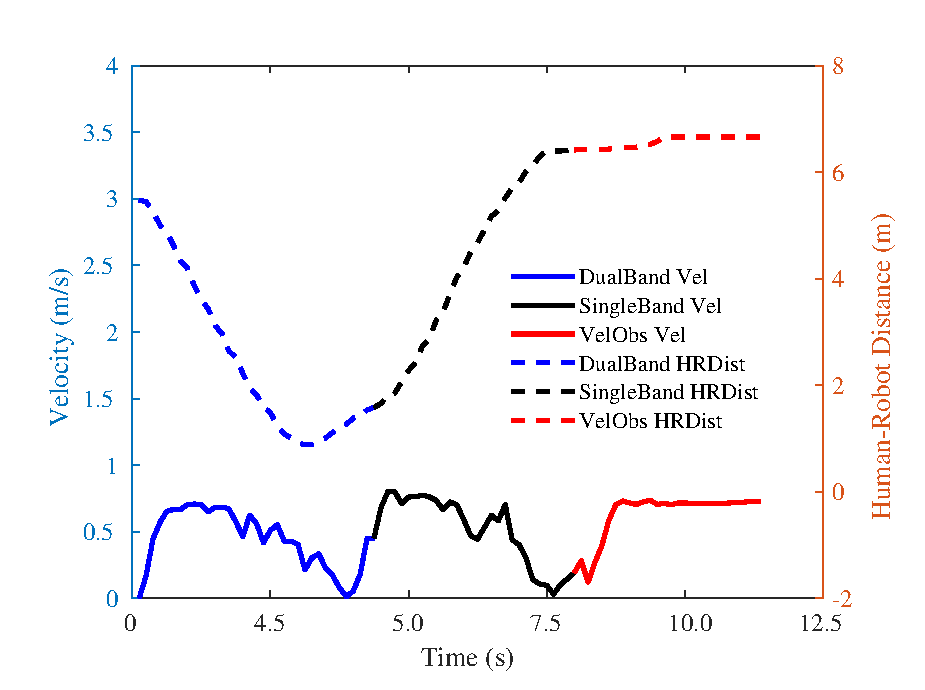
\includegraphics[width=\textwidth]{images/chapter4/door_1}
\end{subfigure}
\hspace{-0.25cm}
\begin{subfigure}{.45\columnwidth}
%   \centering
  % include second image
  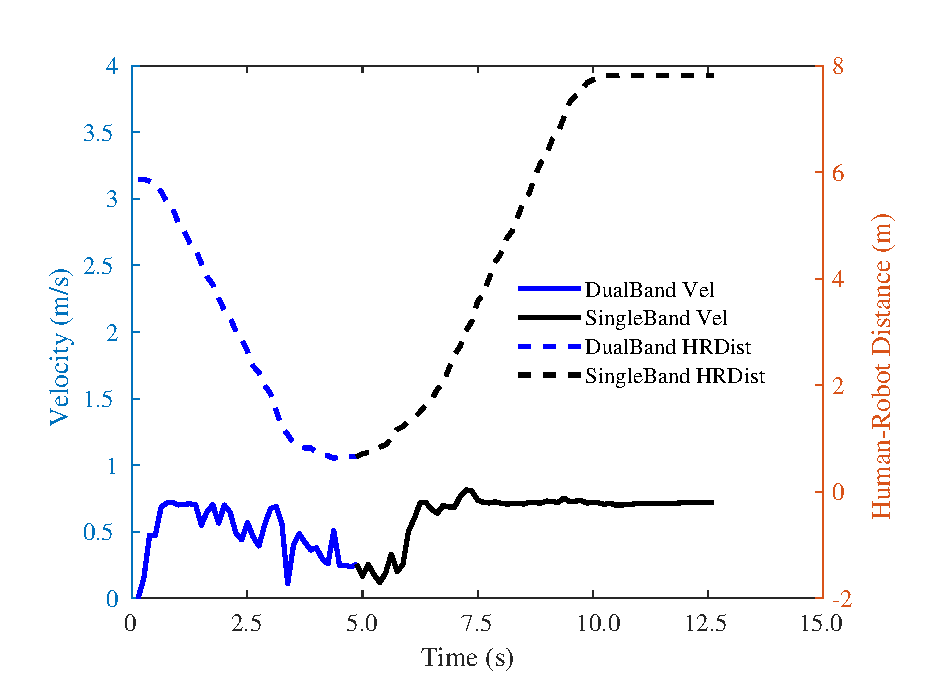
\includegraphics[width=\textwidth]{images/chapter4/door_2} 
\end{subfigure}
\caption{Door crossing scenario in the simulated environment. The human moves towards the door. The robot sees the human and waits on the side of the door (right) until the human crosses.}
\label{fig:door_cross_scene}
\end{figure}
\begin{figure}[h!]
\centering
\begin{subfigure}{.45\columnwidth}
  % include first image
  \includegraphics[width=\textwidth]{images/chapter4/door_3}
\end{subfigure}
\hspace{-0.25cm}
\begin{subfigure}{.45\columnwidth}
%   \centering
  % include second image
  \includegraphics[width=\textwidth]{images/chapter4/door_4} 
\end{subfigure}
\begin{subfigure}{.45\columnwidth}
%   \centering
  % include first image
  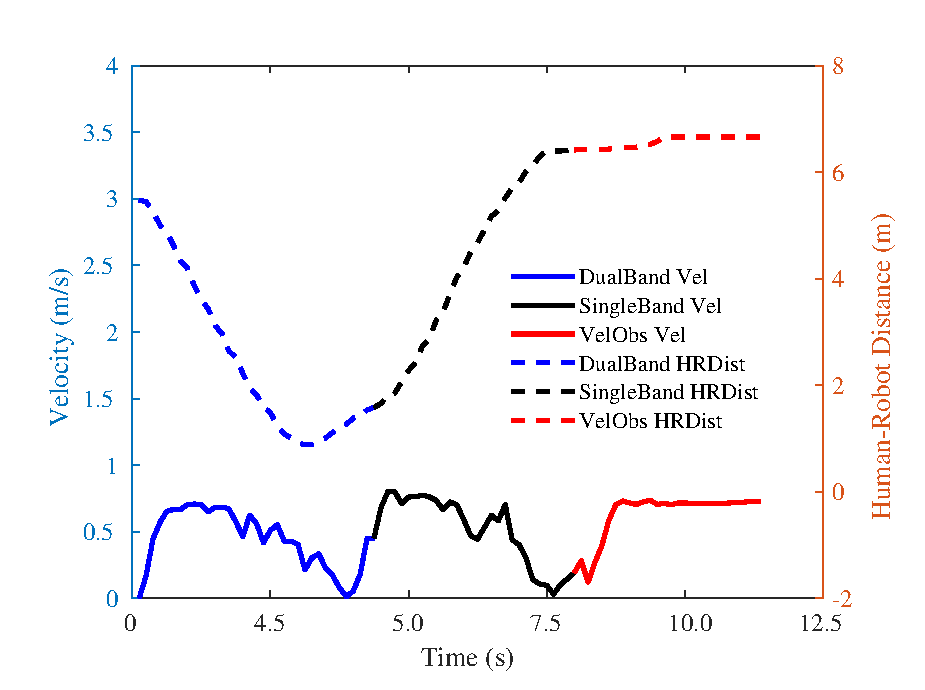
\includegraphics[width=\textwidth]{images/chapter4/door_1.eps}
\end{subfigure}
\hspace{-0.25cm}
\begin{subfigure}{.45\columnwidth}
%   \centering
  % include second image
  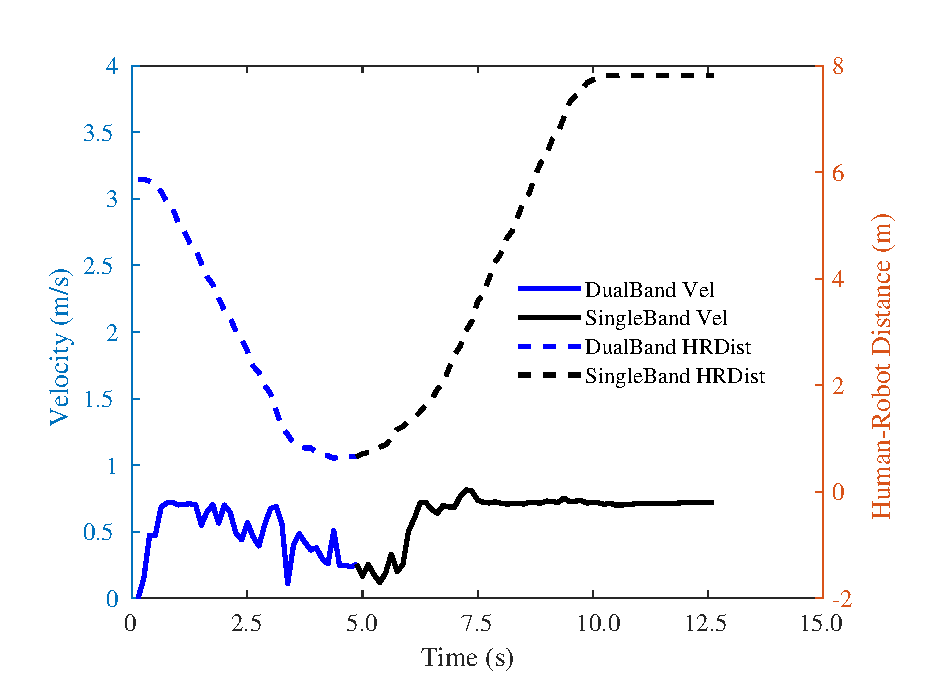
\includegraphics[width=\textwidth]{images/chapter4/door_2.eps} 
\end{subfigure}
\caption{Door crossing scenario in the simulated environment with the static human in two different orientations. Top two pictures show the scenarios in simulation and the planned trajectory of the robot. The bottom two figures show the robot velocity and human-robot distance graphs over time.}
\label{fig:door_cross_static}
\end{figure}

Door crossing is a common situation in many human environments. If two humans try to pass through the same door, one of them has to compromise and clear the way for the other. We have placed the robot running our planning system in the door crossing situation shown in Fig. \ref{fig:door_cross_scene}. The goal of the robot is beside the second human standing in the room, and the system uses \textit{PredictBehind} human path prediction. The left part of the figure shows the simulated scenario and the corresponding trajectories planned for the human and the robot. The simulated human crossing the door was controlled using a joystick and, hence does not move as the planning system expects. The system quickly adapts to these changes and makes the robot clear the way for the human by waiting on the side, as shown in the right part of Fig. \ref{fig:door_cross_scene}. The robot continues to its goal after the human crosses the robot. The planning mode is \textbf{Dual Band} until the human crosses the robot, and then it switches to \textbf{Single Band}.
 
As soon as the robot crosses the door, it faces one more human, but this human is just standing in the same place and does not move. Since the human is static, our system adds the \textit{\textbf{human\_layers}} to the costmaps and re-plans its path. The same scenario is repeated with the second human placed in two different orientations and as shown in Fig. \ref{fig:door_cross_static}. In both scenarios, there is enough space between the wall and the human for the robot to reach its goal, maintaining a safe distance from the human. In the top left scenario of the figure, the human can see the robot, and so the planner makes the robot pass through this space. However, in the second scenario, the human cannot see the robot. Therefore, our planner completely re-plans the path as shown (top right) and makes the robot reach its goal by taking a longer and more visible path. It is due to the added \textit{Human Visibility} layer

Fig. \ref{fig:door_cross_static} also shows the plots corresponding to robot velocity (on the left y-axis) and the distance between the moving human and the robot (human-robot distance) (on the right y-axis) with respect to the time (on the x-axis). Different colours in different portions of the plots correspond to different planning modes of the system, as indicated in the plots. The solid line represents the robot's velocity (Vel), while the dashed line shows the human-robot distance (HRDist). The same conventions are followed across this chapter. From both the graphs (Fig. \ref{fig:door_cross_static} bottom left and right), it can be observed that the Vel decreases as the HRdist decreases. It is a combined effect of several human-aware constraints of our system. However, the \textit{Relative Velocity} constraint plays a major role here. Secondly, it can be seen in the graph of the first scenario (bottom left) that the Vel decreases one more time before the planner changes to \textbf{VelObs} mode. It is because the robot is trying to navigate a narrow space between the human and the wall. This causes the planner to slow down its velocity and check the state of the human. Since the human is static, it shifts to \textbf{VelObs} mode that has little reduced weights for the human-aware constraints and continues its navigation.

\subsection{A Very Narrow Corridor Scene}
This scenario occurs when a long corridor has to be traversed by two humans in opposite directions, and the corridor is wide enough only for a single human. In this case, one of them has to go back and wait for the other to cross. When one of the agents in this scenario is a robot, it becomes a little more complicated as the robot should back off giving priority to the human while taking legible actions. Most of the existing planners either re-plan a long deviation to reach the goal or fail in this complicated situation. A more natural way to handle this would be to clear the way for the human and wait until the human crosses the robot to resume its goal. The \textbf{Backoff-recovery} mode of our system does exactly this. To make the actions more legible, the robot moves back slowly without showing its back until it can go either left or right to clear the way. 
\begin{figure}[!h]
    \centering
    \includegraphics[width=\columnwidth]{images/chapter4/narrow_combined_2.png}
    \caption{Narrow corridor scenario simulated in MORSE. (a) The initial planned trajectory of the robot in \textbf{Dual Band} mode. (b) The robot's way is blocked by the human and the system shits to the \textbf{Backoff-recovery} mode. (c) The robot clears the way for the human and waits on the side until human crosses the robot. (d) The robot continues to its goal in \textbf{Single Band} mode.} 
    \label{fig:narrow}
\end{figure}

The snapshots from the simulated version of this scenario are shown in Fig. \ref{fig:narrow}. Each picture also shows the planned trajectory of the robot in each setting with the \textit{Planning State} behind the robot. This scenario uses the \textit{PredictGoal} human path prediction, and the goal of the robot is on the other side of the corridor. Fig. \ref{fig:narrow} (a) shows the initial situation when the two agents enter the narrow corridor. As the robot can see the human is moving, \acrshort{cohan} operates in \textbf{Dual Band} mode until the human blocks it's way completely. The human agent in this setting is controlled by InHuS~\cite{favier2021intelligent}. As soon as the robot finds itself blocked, it switches to \textbf{VelObs} mode and checks for a possible solution. However, when it cannot find the solution after repeated checks, it switches to \textbf{Backoff-recovery} mode after few seconds ($> \SI{5}{\second}$) as shown in Fig. \ref{fig:narrow} (b). Fig. \ref{fig:narrow} (c) shows the robot waiting for the human to cross the corridor before it can resume its goal. \acrshort{cohan} finally switches to \textbf{Single Band} mode and resumes the robot's navigation to the goal as in Fig. \ref{fig:narrow} (d).

The plots of the Vel and HRDist with respect to time for this scenario are shown in Fig. \ref{fig:narrow_plot}. As the HRDist decreases after a certain threshold, Vel decreases, like in the door crossing scenario (blue part). When the robot switches its mode from \textbf{Dual Band} to \textbf{VelObs}, the robot tries to move in different directions causing the oscillations seen in the plot (red part). In the \textbf{Backoff-recovery} mode, it maintains a constant velocity (green part) and halts, waiting for the human to cross. The human agent of the human simulator starts moving towards the robot as soon as it starts moving back. This explains a near-constant HRDist trend in green. Once the human passes the robot, it resumes its navigation in \textbf{SingleBand} mode (black part).
\begin{figure}[h!]
    \centering
    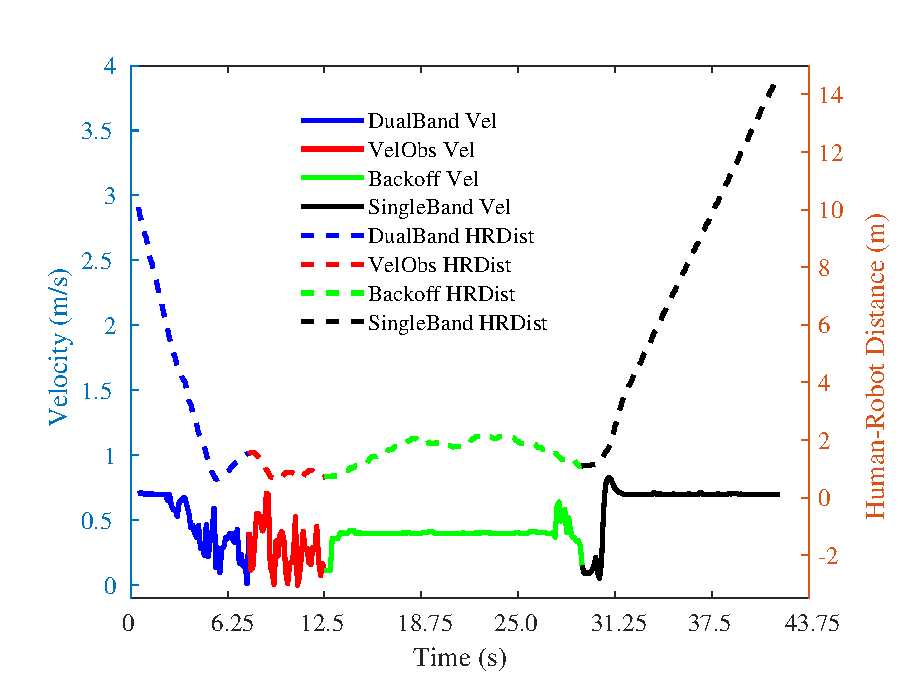
\includegraphics[width=0.8\linewidth]{images/chapter4/nr_cor.eps}
    \caption{Plots of velocity and human-robot distance over time in the Narrow Corridor scenario.}
    \label{fig:narrow_plot}
    \vspace{-0.3cm}
\end{figure}

\subsection{Co-operative Navigation Scenarios}
We have simulated three other scenarios in MORSE where cooperation is needed for successful navigation. These three scenarios are called `Pillar Corridor', `Wide Corridor' and `Open Space'. Fig.~\ref{fig:other_scenes} shows the snapshots of these scenarios (top part) and part of the trajectory planned by \acrshort{cohan}. In all three scenarios, human and robot goals are behind each other, and they start navigation at the same time. In the Wide Corridor scenario, 
\acrshort{cohan} uses \textit{PredictBehind} path prediction for the human, and hence the human's goal is estimated to be at the back of the robot's initial position. The path generated using this goal is then used to plan the human trajectory. In this case, we use this planned human trajectory to control the human, and thus it represents the ideal scenario for the planner. This scenario and its corresponding Vel and HRDist plots are shown in Fig. \ref{fig:other_scenes} (b). We can see from these plots that the Vel decreases as the HRDist decreases, but it never goes to zero as the human is behaving ideally. We can also see the shift from \textbf{Dual Band} to \textbf{Single Band} mode as soon as the human crosses the robot. This is true for all three cases. 
\begin{figure}[!h]
\centering
    \begin{subfigure}{\textwidth}
    \centering
      \includegraphics[width=0.9\columnwidth]{images/chapter4/co-operative_scenes}
    \end{subfigure}
    \begin{subfigure}{.3\columnwidth}
      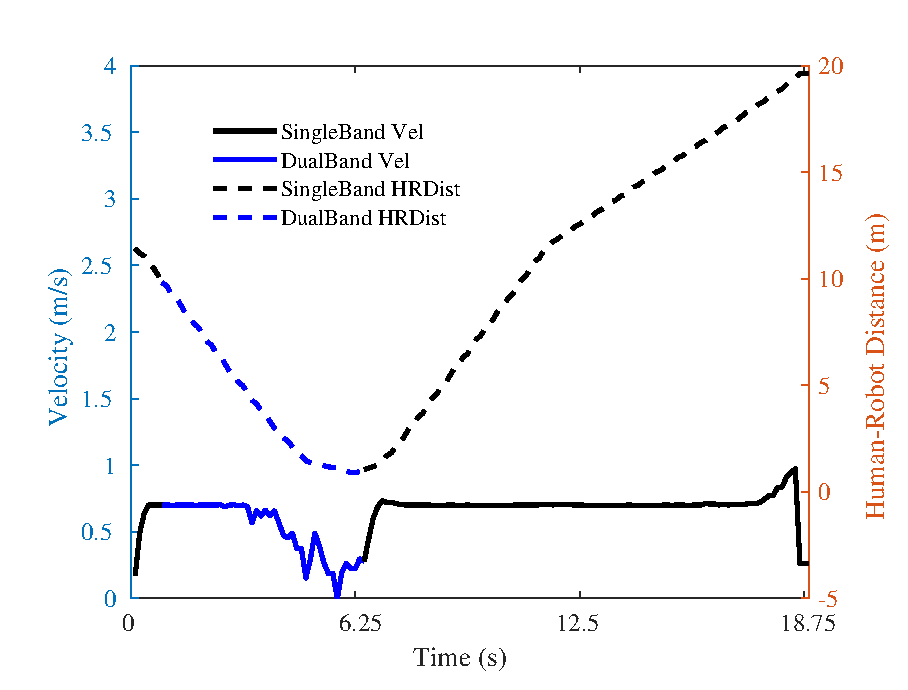
\includegraphics[width=\linewidth]{images/chapter4/p_cor.eps}\caption{Pillar Corridor}
    \end{subfigure}
    \hspace{-0.3cm}
    \begin{subfigure}{.3\columnwidth}
      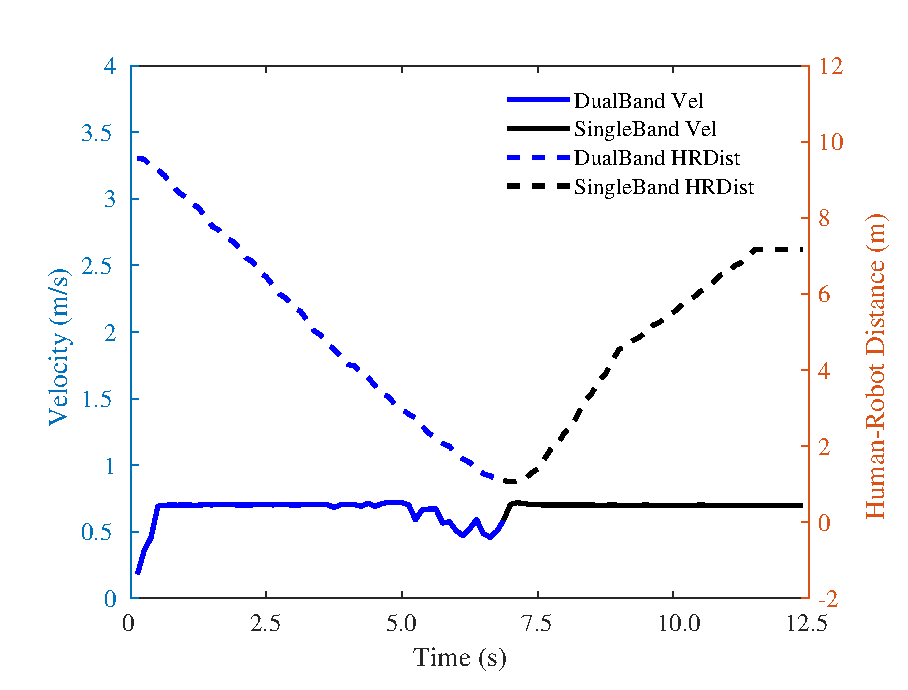
\includegraphics[width=\linewidth]{images/chapter4/n_cor.eps}
      \caption{Wide Corridor}
    \end{subfigure}
    \hspace{-0.3cm}
    \begin{subfigure}{.3\columnwidth}
      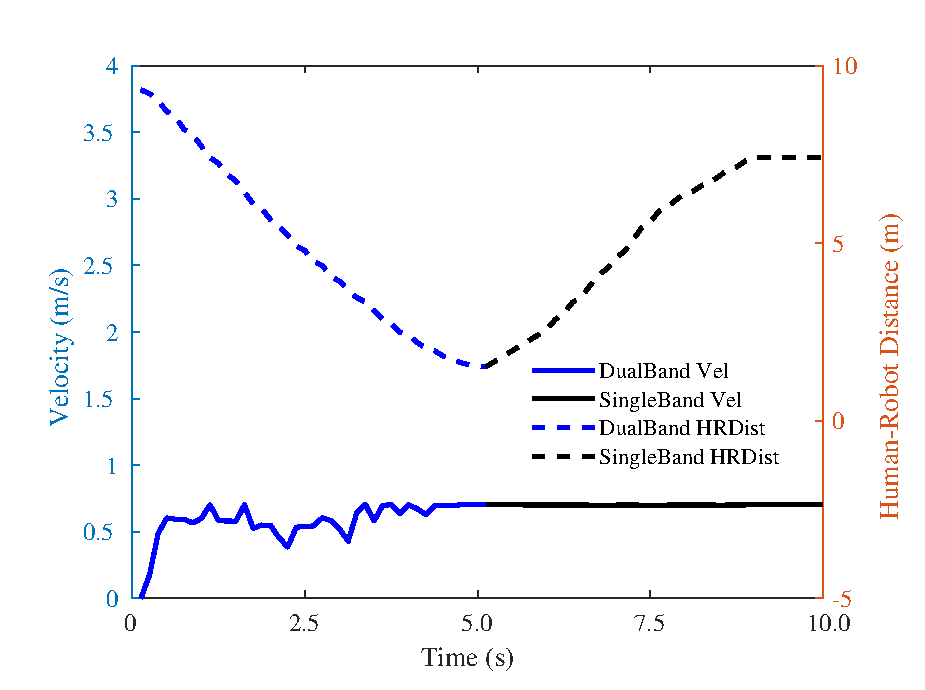
\includegraphics[width=\linewidth]{images/chapter4/w_cor.eps}
      \caption{Open Space}
    \end{subfigure}
    \caption{(a) A corridor with pillars, wide enough for only one agent at the side of the pillar. (b) A wide corridor where the two agents have enough space to cross each other maintaining safe distances. (c) An open space scenario where the robot has enough space to avoid and show its intention to the human well in advance. In (a), (b) and (c), the plots of robot's velocity and human-robot distance over time are shown below the scenario.}
    \label{fig:other_scenes}
    \vspace{-0.4cm}
\end{figure}

In the other two scenarios, the human agent was controlled by InHuS, and the system uses \textit{PredictGoal} human path prediction. The Vel and HRDist plots for these scenarios are shown in Fig. \ref{fig:other_scenes} (a) and (c). From the plots of the Pillar Corridor in Fig. \ref{fig:other_scenes} (a), we can see that the robot's velocity decreases rapidly and momentarily goes to zero. This occurs as \acrshort{cohan} plans proactively and makes the robot wait behind the pillar to let the human cross. This scenario highlights the priority given to humans over the robot in our planning system. The plots of the Open Space scenario in Fig.~\ref{fig:other_scenes} (c) show a jerky velocity profile in the \textbf{Dual Band} mode and a smooth one in \textbf{Single Band} mode. However, the speed does not go down significantly. As the robot has enough space to move away from the human and continue its navigation at high speed, \textit{Relative Velocity} constraint pushes the robot to a larger distance from the human. Hence, the jerky Vel profile is due to the directional changes in the velocity. Note that the HRDist, in this case, is always more than \SI{1.5}{\metre}, thanks to the \textit{Relative Velocity} constraint. By looking at the initial trajectory generated by \acrshort{cohan} in Fig.~\ref{fig:other_scenes} (c), it is clear that the robot chooses to go to the left very early during its navigation, and we can argue that this intention show makes the robot's trajectory legible to the human.

\subsection{Robot in a Crowd}
\begin{figure}[h!]
    \centering
    \includegraphics[width=0.9\columnwidth]{images/chapter4/pedsim_new}
    \caption{The robot running CoHAN system in the PedSim ROS pedestrian simulator. The robots planned trajectory and the predicted trajectories of the two nearest humans in \textbf{VelObs} mode are shown.}
    \label{fig:pedsim_ros}
\end{figure}

For this experiment, we tuned the parameters of \acrshort{cohan} and tested it in a simulated crowd. For the simulation of crowds, we used the PedSim ROS simulator, and \acrshort{cohan} is run completely in the \textbf{VelObs} mode. Therefore, the human path prediction by default is set to \textit{PredictVelObs}, which is a linear prediction methodology, as previously mentioned. Fig.~\ref{fig:pedsim_ros} shows two snapshots from the tests. The robot adds elastic bands to two of the nearest humans in the environment and successfully navigates the crowd generated by the simulator (shown in video\footnote{\url{https://youtu.be/DB_8HpjngJ4}\label{cohan_video}}). Further, it can be seen that the robot proactively clears the way for PedSim agents while navigating in the corridor, as shown in the snapshot to the right in Fig. \ref{fig:other_scenes}. Even though \acrshort{cohan} was mainly designed for indoor navigation scenarios, this example shows how it can be tuned and scaled to scenarios with a large number of humans. The choice of proactively planning only for two of the nearest humans did not affect the navigation performance as the system was able to quickly switch between different humans.  

\subsection{Comparison with Another Human-Aware Planner}
\begin{table*}[ht!]
    \centering
    \begin{tabular}{|c|c|c|c|}
    \hline
     & \multicolumn{3}{c|}{CoHAN} \\
    \cline{2-4}
    Experiment & \textit{Path Length} $(m)$ & \textit{Total Time} $(s)$ & \textit{Min  HRDist} $(m)$\\
    % & \textit{Path Length} $(m)$ & \textit{Total Time} $(s)$ & \textit{Min  HRDist} $(m)$\\
    \hline
    \textit{Open Space} & 9.23 & \textbf{16.01} & \textbf{1.29} \\
    % & \textbf{8.7892} & 24.7683 &0.9508\\
    \hline
    \textit{Narrow Passage} & 9.73 & \textbf{17.80} & 0.71\\ 
    % & \textbf{9.4017} & 27.1633 & \textbf{0.935}\\
    \hline
    \textit{Pillar Corridor} & 19.11 & \textbf{31.46} & \textbf{0.89} \\
    % & \textbf{18.4489} & 52.9417 & 0.7589\\
    \hline
    \textit{Narrow Corridor} & \textbf{23.54} & \textbf{48.38} & \textbf{0.66}\\
    % & - & - & -\\
    \hline
    & \multicolumn{3}{c|}{TPF}\\
    \cline{2-4}
    \hline
    \textit{Open Space} & \textbf{8.79} & 24.77 &0.95\\
    \hline
    \textit{Narrow Passage} & \textbf{9.40} & 27.16 & \textbf{0.93}\\
    \hline
    \textit{Pillar Corridor} & \textbf{18.45} & 52.94 & 0.76\\
    \hline
    \textit{Narrow Corridor} & - & - & -\\
    \hline
    \end{tabular}
    \caption{Mean values of the metrics over 10 repetitions in four different contexts. TPF failed in the Narrow Corridor case.}
    \label{results_cohan}
\end{table*}
In order to check the repeatability of our system and evaluate its performance with respect to the existing human-aware navigation planners, we have selected four different simulated scenarios and repeated the same experiment 10 times in each of the scenarios. The scenarios we considered here include Open Space, Narrow Passage (similar to the one in Chapter.~\ref{chap:3}), Pillar Corridor and Narrow Corridor. The human in all these scenarios is controlled by InHuS. In all these scenarios, our system produced consistent results over the repetitions with similar paths. Further, we compared it with the human-aware navigation planner presented in \cite{kollmitz2015time} that was designed for indoor home context. This system uses \textit{Timed Path Follower} (TPF) as its local planner, and its trajectory is highly dependant on the path produced by its global planner, \textit{Lattice Planner}. Note that our comparison was limited to only one planner as not many human-aware planners are available openly for indoor contexts. This planner was also made to run repeatedly 10 times in the above four scenarios. However, in the Narrow Corridor case, this planner failed to complete the navigation, and the robot got stuck in front of the human as the \textit{Lattice Planner} could not find a path.

We used three different metrics to present the comparisons between these two planners, the total length of the path taken, the total time to complete the scenario and the minimum human-robot distance that the planner encountered while executing each scenario. The average over the 10 runs is taken and presented in Table~\ref{results_cohan}. Note that the total time taken by the TPF is greater as its linear velocity was limited by the planner, even though the same velocity and acceleration limits of the robot were provided to both planners. In terms of the total path length, TPF always followed a lesser distance compared to \textit{\acrshort{hateb}}. This is because \textit{\acrshort{hateb}} took the larger deviations to either show intentions (in Open Space) or a clear path for the human (Pillar Corridor and Narrow Passage). However, in the Narrow Passage case, TPF produced better behaviour by waiting for the human to cross while \textit{\acrshort{hateb}} blocked the way for a bit before clearing the way for the human\footnote{\url{https://youtu.be/DB_8HpjngJ4}}. This can also be seen by comparing the minimum human-robot distance in this case. Finally, in terms of the minimum human-robot distances, \textit{\acrshort{hateb}} varies widely, as it handles each case differently. If space is available, it takes a greater distance than TPF, otherwise, it slows down the robot's velocity and approaches a little closer to the human. In TPF, this metric produces similar results in two of the three scenarios. In the Pillar Corridor, this metric has a lesser value compared to \textit{\acrshort{hateb}} as the robot goes towards the wall to the opposite side of the pillar and waits instead of going behind the pillar. 

\section{Real-world Experiments with CoHAN}
\label{real_chap4}
\begin{figure}[h!]
    \centering
    \includegraphics[width=0.9\columnwidth]{images/chapter4/wide_real.jpg}
    \caption{CoHAN running on Pepper in open space. The pictures shows the planned trajectory of the robot around the moving human.}
    \label{fig:real_exp}
\end{figure}

\begin{figure}[h!]
    \centering
    \includegraphics[width=0.9\columnwidth]{images/chapter4/backoff_real.jpg}
    \caption{Testing \textbf{Backoff-recovery} on the real robot. As the human blocks the way, the robot cannot find any solution to move, and CoHAN makes the robot back-off and wait for the human to pass.}
    \label{fig:real_backoff}
\end{figure}
We deployed \acrshort{cohan} on a real robot platform, Pepper\footnote{\url{https://www.ald.softbankrobotics.com/en/pepper}} to conduct some real-world experiments in our lab. For human detection and tracking, we used the OptiTrack\footnote{\url{http://www.optitrack.com/}} motion capture system and published the positions and velocities of the tracked humans at 10 Hz. The localization of the robot is done in the same manner as in Chapter.~\ref{chap:3} using Aruco markers. However, during these experiments, the odometry of the robot shifted a lot, and even a small run drifted the robot far from its original position. Even with this bad odometry, we were able to capture two good runs, one in an open space and the other showing the \textbf{Backoff-recovery} in a narrow corridor.

Fig.~\ref{fig:real_exp} shows the instances from the run in open space. The figure also shows the trajectories of the robot at the bottom of each instance. In this scenario, as the robot starts moving towards the goal, the human approaches faster than the robot anticipated. He comes close to the robot at the crossing point, but the robot immediately backs off and clears the way for the human. It slows down for a moment before re-planning its trajectory to the goal, as seen in the video\footnote{\url{https://youtu.be/DB_8HpjngJ4}}. The wrong estimate could be due to bad odometry or network delays. The second run shown in Fig. \ref{fig:real_backoff} shows instants from the test of \textbf{Backoff-recovery} mode in \acrshort{cohan}. The human stands in the corridor blocking the robot's way. The planner starts in \textbf{Dual Band} mode and finally switches to \textbf{Backoff-recovery} mode as there is no solution. The robot slowly backs off and clears the way for the human by moving to the left side of the corridor, as seen in Fig. \ref{fig:real_backoff}. The human then moves out of the corridor and clears the way for the robot.

\section{Multi-context HAN and CoHAN}\label{discussion_chap4}
In this section, we present a discussion on HAN planning with multiple planning modalities and how this coupled with the situation assessment, can address multiple human-robot navigation contexts. We also present a brief discussion on how \acrshort{cohan} addresses some of these contexts and talk about the possible extensions for \acrshort{cohan}.

\subsection{Modality based HAN Planning}
Some of the early works in HAN with multiple modes of planning like \cite{qian2013decision, mehta2016autonomous} used \acrshort{pomdp} based policies to choose different actions to avoid the freezing robot problem or the frequent re-planning. They show how having multiple policies benefits robot navigation and also increases the success rate. The increase in success rate does not necessarily mean that the navigation is acceptable and legible to the humans in the environment. We believe that if this multi-policy planning could be coupled with social norms of the environment, the resultant system could offer legible robot navigation among humans with high success rates. \acrshort{cohan} is one such approach where situation assessment and decision-making are coupled with a complete HAN planning system and offers some interesting planning modalities. Unlike the previous works, we do not use a \acrshort{pomdp} based approach but rather propose engineered ways to analyse situations and shift between modalities. A very recent work similar to our approach is presented by Banisetty  \cite{banisetty2020deep}. It uses a multi-objective optimization based local planner like ours and employs a deep learning based situation assessment module. Compared to the previous works with only multiple modes of planning, \acrshort{cohan} and the HAN system by \cite{banisetty2020deep} use situation assessment not only to successfully navigate the robot but also to add socially compliant behaviour to the navigation policies. These frameworks can hence be used to solve multiple human-robot navigation contexts.

\subsection{Multi-Context HAN Planning using Mode Shifting}
Classical robot navigation can be generalized, and a planning scheme might work for different contexts without any modifications. On the other hand, HAN requires addressing different \acrshort{hri} contexts and hence, possibly requires different planning strategies. If these strategies can be employed as planning modalities, the frameworks can be used for solving multiple human-robot contexts. This approach is quite new, and limited research exists in this field. The work by \cite{banisetty2020deep} presented above uses multi-objective optimization and geometric reasoning to address the multi-context navigation of a robot in human environments. It presents some very interesting contexts and scenarios that were addressed by combining situation assessment with HAN planning. Our approach, \acrshort{cohan}, is a parallel work and addresses multi-context navigation in a similar fashion but uses proactive planning with an engineered situation assessment loop. Further, our system offers a variety of parameter settings that can choose prediction mode, the human-aware constraints to be used and tuning over these costs. Even the planning can be restricted to only one of the three planning modes (except \textbf{Backoff-recovery}). Hence, it can be further extended to many kinds of human-robot contexts by properly choosing the parameters and with simple tuning. With the addition of the costmap layers around the static humans, this framework can handle most of the scenarios presented in \cite{banisetty2020deep}. \acrshort{cohan} already uses some geometric reasoning to better understand the intricate \acrshort{hri} contexts with a human, and it can be easily extended to address group interactions.

\subsection{CoHAN in Multiple Human-Robot Navigation Contexts}
Currently, \acrshort{cohan} is developed to address intricate human-robot scenarios that often occur in indoor environments like offices or labs. The added costmap layers and updated human-aware constraints provide promising results in situations like joining or leaving a group, over-taking a human from behind, various types of human-robot crossing scenarios at doors or in corridors and general HAN in wide spaces with few humans. With small modifications in the parameters, it can even be extended to crowded scenarios, as shown in the section~\ref{results_chap4}. Still, there are \acrshort{hri} contexts \acrshort{cohan} cannot address presently, like following or accompanying humans \cite{repiso2017line}, approaching humans \cite{khambhaita_hfr_2016} or taking an elevator with humans. We plan to extend \acrshort{cohan} to address the scenarios mentioned above and modularise the design of \acrshort{cohan} so that customized human-robot navigation contexts can be added easily. The approach modality is already studied with some implementations in \acrshort{hateb}, and so the next step would be completely integrating this modality into \acrshort{cohan}. For the elevator scenario, a new custom modality needs to be developed such that the robot is allowed to violate the human proxemics but still acts in a human-friendly manner. Finally, the existing literature on the person-following robot can help design another modality for \acrshort{cohan}.

\section{Conclusion}\label{conclude_chap4}
In this chapter, we proposed a new HAN planner that can handle a variety of human-robot contexts. It was able to handle both outdoor crowd scenarios and indoor intricate scenarios, thanks to the different planning modes and tunable parameters. These planning modes are at the control level and, hence, differ from higher level modes as used in \cite{mehta2016autonomous}. Consider the \textbf{Backoff-recovery} mode, for example, instead of going into the corridor, the robot could have stopped (or back off) as soon as it sees a person, or if the robot has progressed more than the human, the human can go back and let the robot go. By employing a higher level planner over our system, this case can be handled much more efficiently, but our focus is on providing this feature at the control level. We introduced \textit{Human Safety} and \textit{Human Visibility} layers into the system through costmaps to address the static human scenarios. For handling the dynamic humans, we have used a variety of human-aware constraints in \textit{\acrshort{hateb}} along with visibility and planning radius. The proposed system also provided different types of human path prediction methods. We have proposed two new human-aware constraints in addition to the previous ones present in \textit{\acrshort{hateb}} to offer a more legible trajectory. Further, our system was evaluated in a variety of simulated scenarios and presented both qualitative and quantitative results. Finally, real-world tests on a robotic platform were presented.

One of the major limitations of our system could be computational complexity as it performs optimization in each control loop. However, it does not affect the real-time performance of the robot in \textbf{Single Band} and \textbf{Backoff-recovery} modes (10Hz). In the other modes, it may lead to a little reduced control rate (8-9 Hz), however still in real-time. One of the immediate future works is to develop a higher-level planner on top of our system to handle the contexts more efficiently and to include more contexts like following or accompanying a human. Currently, the system is not designed for handling groups of people differently, and we plan to include it in the future version of the system. 
 
The situations presented in this chapter and the possible extensions discussed above only deal with the humans that are currently visible and are within the planning environment. Designing a HAN system for handling all the scenarios that arise in such a setting is already complicated and requires further studies and new planning methodologies. However, there is no work addressing the humans that might emerge into the planning scene and can disturb the current motion of the robot. A complete HAN system should proactively anticipate such possibilities and be prepared instead of freezing in such scenarios. So, in the next chapter, we introduce the concept of `invisible humans' to HAN to handle such scenarios.
